\section{The PDF Trust Chain \note{1.5pp}}
\label{sec:trust-chain}

\subsection{Trust Chains in General}
The term \emph{Trust Chain} (or ``Chain of Trust'') is used in multiple contexts, e.g.,
\emph{digital certificates}: a sequence of certificates signing certificates,
starting with a root certificate;
\emph{supply chain}: a product is no more reliable or secure than its
outsourced components;
\emph{trusted boot}: unless the bootloader is correct and non-malicious,
there can be no possibility of the operating system being the same;
\emph{software stacks}: upper layers are dependent upon lower layers (such as
system libraries) and vulnerabilities at the lower layers affect all higher layers.

The common idea is having layers
that rely on lower layers for their validity
(or components that rely on sub-components, etc.)
And the key lesson being,
{\bf{if a single layer of the trust chain 
  is flawed or suborned, then every layer relying on it
  is no longer capable of being trusted.}}

\mtnote{I use 'layer' in this subsection, but hereafter I'll be using
  'stage' (not phase/component/etc) for our concrete instance in PDF.}

\subsection{The Trust Chain of a PDF Parser}

% In \cref{sec:pdf-challenges}, we elaborated on the challenges of PDF.
% Parsing data-formats has a long history and many solutions ...
% Parsing formal languages also has a long history and many solutions ...
% PDF has aspects of both: this makes PDF challenging.
% But PDF ``parsing'' is not merely a matter of harder [difference of degree]
% but intrinsically more complex [a difference of kind!]:

\begin{figure}[t]
  \centering
  \begin{lstlisting}
    +-----------------------------------------------------+
    | 1. Find & parse header and trailer                  |<-- File
    +-----------------------------------------------------+
                       | offsets + ...
                       v
    +-----------------------------------------------------+
    | 2. Find & parse incremental updates                 |<-- File
    +-----------------------------------------------------+
                       | list of XRef maps
                       v
    +-----------------------------------------------------+
    | 3. Merge incremental updates                        |
    +-----------------------------------------------------+
                       | XRef map
                       v
    +-----------------------------------------------------+
    | 4. Transform XRef map to object map (DOM)           |
    |    1. Parse uncompressed objects                 <--+-- File
    |    2. Decode streams & preprocess object streams <--+-- File
    |    3. Resolve type 2 object references           <--+-- File
    +-----------------------------------------------------+
                       | Object map (DOM)
                       v
    +-----------------------------------------------------+
    | 5. Validate candidate DOM                           |
    +-----------------------------------------------------+
                       | Object map (DOM)                                    
                       v
    +-----------------------------------------------------+
    | 6. Render DOM                                       |
    +-----------------------------------------------------+
                       | 
                       v
  \end{lstlisting}
  % 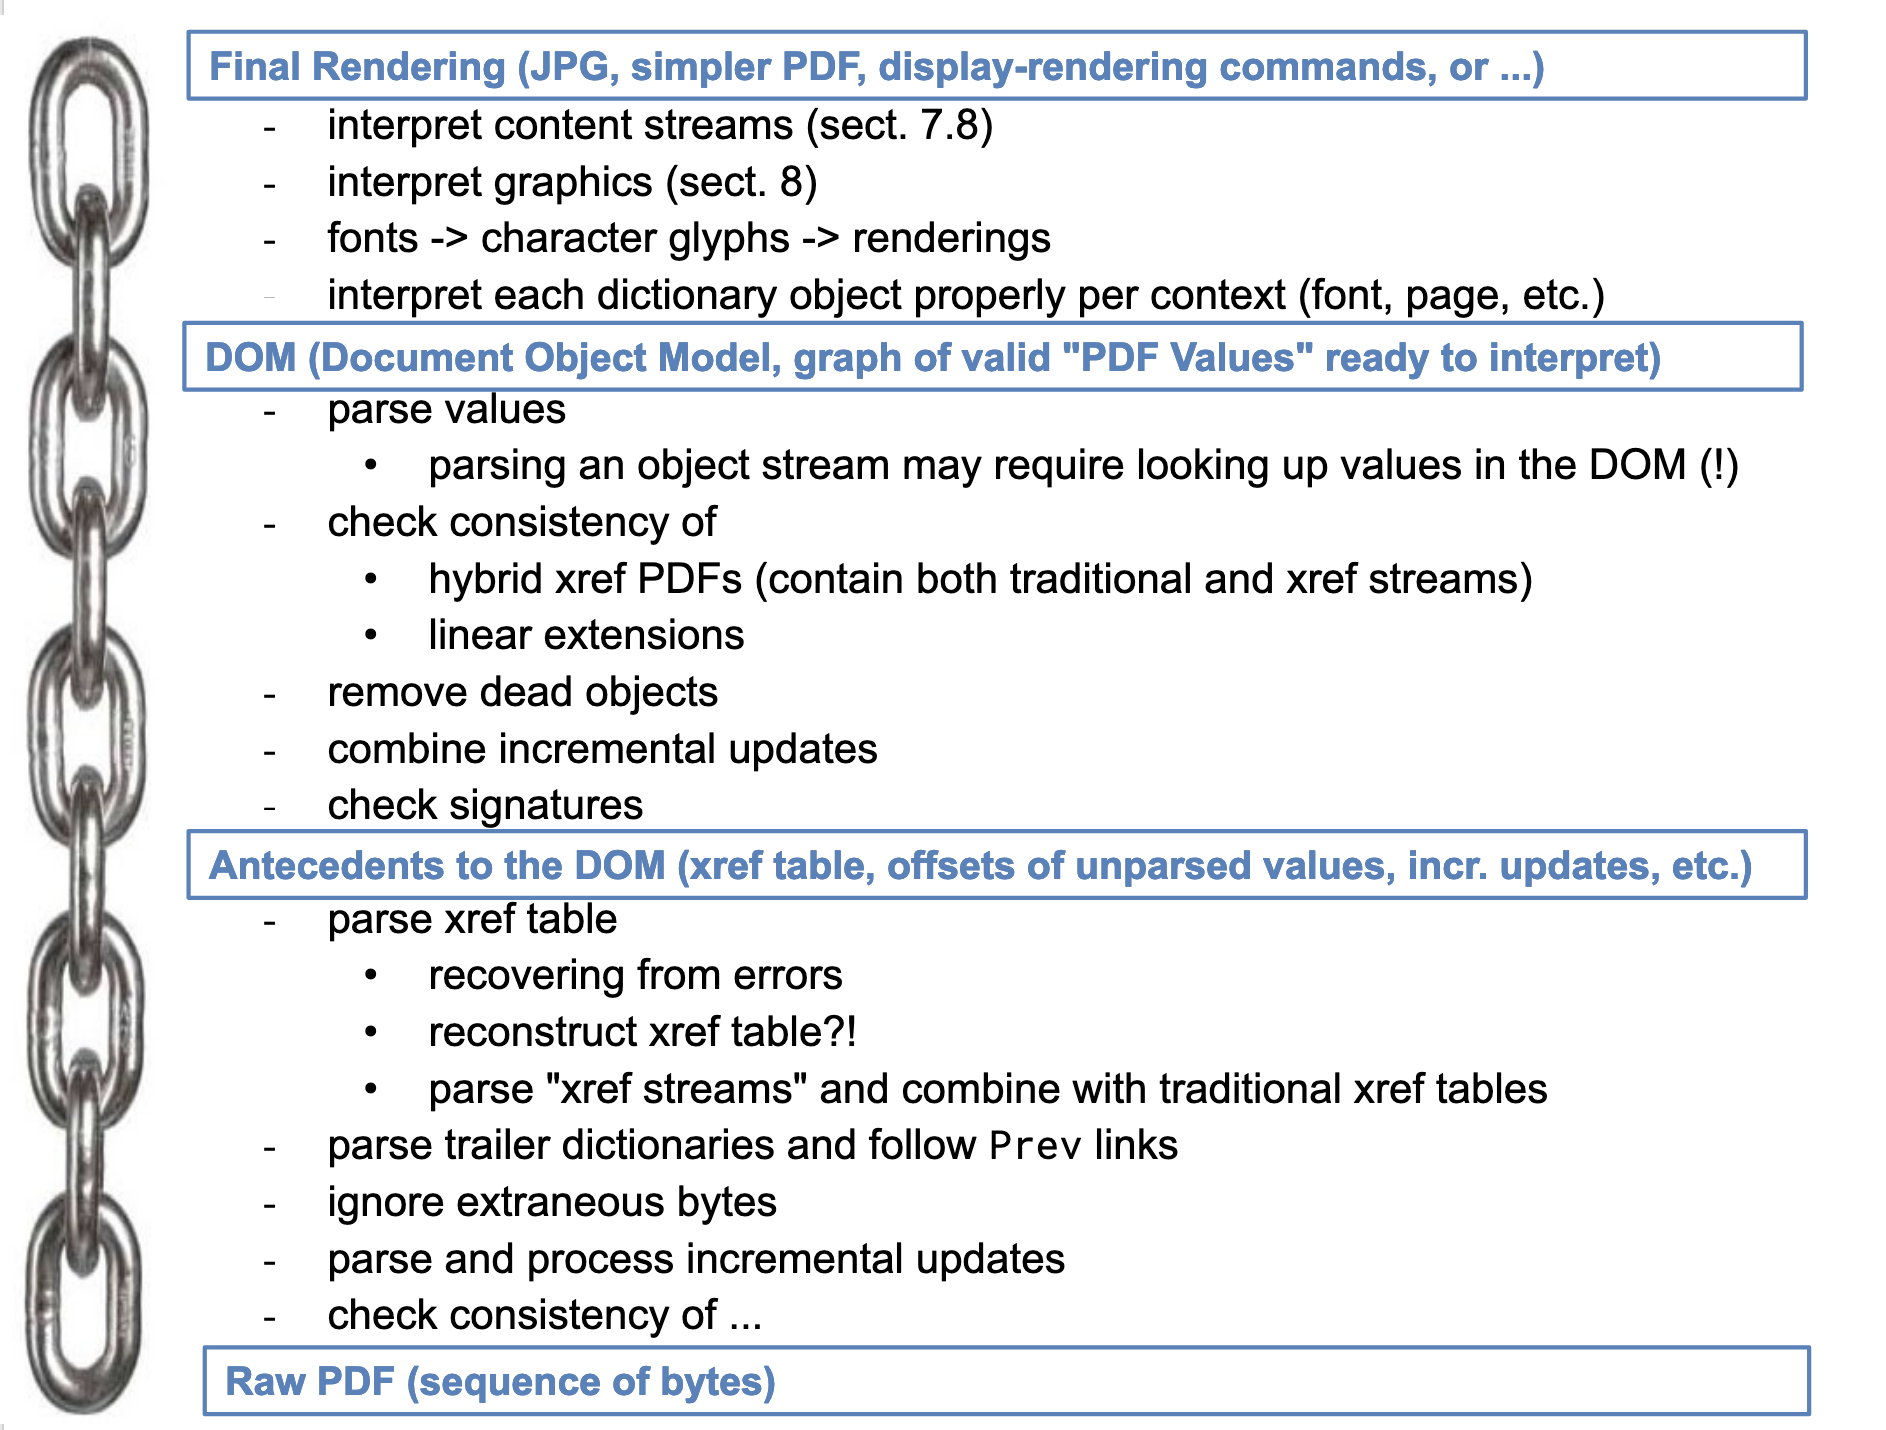
\includegraphics[width=0.8\linewidth]{figures/trustchain-diagram.png}
  \caption{Stages of PDF Parsing (the Trust Chain)}
  \mttodo{un-ascii-ify diagram}
  \label{fig:pdf-trust-chain}
\end{figure}

We have touched upon the complexities of parsing
PDF, but to appreciate these, one has to understand the
dependencies and interactions between the features.
In \cref{fig:pdf-trust-chain} we show the main stages diagrammatically.
To briefly sketch what's going on in each stage:
\begin{itemize}
\item Stage 1: Find and parse both the PDF header and the PDF trailer.
\item Stage 2: Find and parse all the incremental updates.  Note that this stage
  uses the file offsets from Stage 1 in order to know \emph{where} to find the
  incremental updates
\item Stage 3: This stage does no further reading of the file.
\item Stage 4: Transform XRef map to object map. This stage is complex and
  requires three stages, each of which does further file input and parsing.
  Further details are in \cref{sec:specifying}.
  If all goes well, we have a syntactically correct DOM.
\item Stage 5: Validate candidate DOM.  This stage takes the candidate DOM and
  verifies that it represents a sensible Document Tree per the PDF Standard.
  E.g., all indirect objects are in the candidate DOM, no unexpected recursion,
  etc.
\item Stage 6: Render.  Here we render the validated DOM, or parts thereof, to
  whatever display or graphic format we choose.
\end{itemize}

Note that stages 2, 4.1, 4.2, and 4.3
all use inputs from the previous stage to determine where and
how to further parse segments of the PDF input file.
An error in an earlier stage will always affect the output of later stages,
but errors that percolate into these stages can cause parsing of the wrong data.
%
The attentive reader will note that we have another instance of a \emph{Trust
Chain}.  The subsequent stages of the parsing process are \emph{completely
dependent} upon the earlier stages to properly parse and interpret the PDF
file.

Note this: an implementation \emph{might} merge stages 2, 3, 4.1, 4.2, 4.3 into
a single stage and give a \emph{semblance} of simplicity, our argument in what
follows---particularly in \cref{sec:single-pass-problems}---is that such an
implementation will be overly complex and result in a nearly insurmountable task
to assure that such an implementation is actually implementing the standard
and terminating for all input files.

We think it is important to understand PDF parsing in terms of this
\emph{Trust Chain} because
%
(1) it highlights the presence of the many ``dependent'' stages
in PDF processing.
%
(2) it highlights the importance of ensuring the pre-DOM parsing, data integrity relationships and
computation (the base of our Trust Chain) is correct and secure.
%
(3) it reminds us that the integrity of the DOM cannot be verified
independently of the lower levels.
%
(4) it illustrates that PDF parsing, although uniquely complex, is an instance of
a general concept.

Although verifying Stage 5 is both difficult and tedious
(\pwtodo{...; say something re the Arlington DOM model? a paper?})
and the Render stage has many complications of its own (e.g., fonts are
a special challenge), we will focus on stages 1-4.
We refer to these stages as pre-DOM parsing/computation; if anything
goes wrong pre-DOM---and lots can go wrong---there's hell to pay. \mtnote{?!}
